\begin{tikzcd}[column sep=1.5em,row sep=1.4em]
\mathbb A^1\arrow[d]\arrow[dd,bend right=55,"{x\mapsto x^2}"']&
{\begin{tikzpicture}[baseline=0,x=1cm,y=1cm,font=\small]
\draw (-1.8,.4)..controls (-.3,.3) and (.3,-.3)..(1.8,-.4);
\draw (-1.8,-.4)..controls (-.3,-.3) and (.3,.3)..(1.8,.4);
\fill[red] (1.4,.34) circle (1.6pt);\node[red,above] at (1.4,.34) {$x$};
\fill[red] (1.4,-.34) circle (1.6pt);\node[red,below] at (1.4,-.34) {$-x$};
\node[red,above] (noid) at (-.2,.7) {此处不等同};\draw[red,->] (noid.south)--(0,.04);
\node[red,right] at (1.8,0) {等同};
\end{tikzpicture}}\arrow[d]\\
X\arrow[d]&
{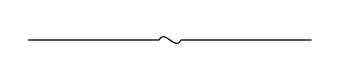
\begin{tikzpicture}[baseline=0,x=1cm,y=1cm]
\draw (-1.8,0)--(-.14,0)..controls (-.07,.15) and (.07,-.15)..(.14,0)--(1.8,0);
\end{tikzpicture}}\arrow[d]\\
\mathbb A^1&
{\begin{tikzpicture}[baseline=0,x=1cm,y=1cm]\draw (-1.8,0)--(1.8,0);\end{tikzpicture}}
\end{tikzcd}
